%%%%%%%%%%%%%%%%%%%%%%%%%%%%%%%%%%%%%%%%%
% Professional Formal Letter
% LaTeX Template
% Version 1.0 (28/12/13)
%
% This template has been downloaded from:
% http://www.LaTeXTemplates.com
%
% Original author:
% Brian Moses (http://www.ms.uky.edu/~math/Resources/Templates/LaTeX/)
% with extensive modifications by Vel (vel@latextemplates.com)
%
% License:
% CC BY-NC-SA 3.0 (http://creativecommons.org/licenses/by-nc-sa/3.0/)
%
%%%%%%%%%%%%%%%%%%%%%%%%%%%%%%%%%%%%%%%%%

%----------------------------------------------------------------------------------------
%	PACKAGES AND OTHER DOCUMENT CONFIGURATIONS
%----------------------------------------------------------------------------------------

\documentclass[11pt,a4paper]{letter} % Specify the font size (10pt, 11pt and 12pt) and paper size (letterpaper, a4paper, etc)

\usepackage{graphicx} % Required for including pictures
\usepackage{microtype} % Improves typography
\usepackage{gfsdidot} % Use the GFS Didot font: http://www.tug.dk/FontCatalogue/gfsdidot/
\usepackage[T1]{fontenc} % Required for accented characters

% Create a new command for the horizontal rule in the document which allows thickness specification
\makeatletter
\def\vhrulefill#1{\leavevmode\leaders\hrule\@height#1\hfill \kern\z@}
\makeatother

%----------------------------------------------------------------------------------------
%	DOCUMENT MARGINS
%----------------------------------------------------------------------------------------

\textwidth 6.75in
\textheight 9.25in
\oddsidemargin -.25in
\evensidemargin -.25in
\topmargin -1in
\longindentation 0.50\textwidth
\parindent 0.4in

%----------------------------------------------------------------------------------------
%	SENDER INFORMATION
%----------------------------------------------------------------------------------------

\def\Who{} % Your name - Presidente do Conselho Monetário Nacional
\def\Where{Department of Mathematics} % Your department/institution
\def\Address{123 Broadway} % Your address
\def\CityZip{Berkeley CA 12345} % Your city, zip code, country, etc
\def\Email{E-mail: j.smith@berkeley.edu} % Your email address
\def\TEL{Phone: (000) 111-1111} % Your phone number
\def\URL{URL: http://www.johnsmith.com} % Your URL

%----------------------------------------------------------------------------------------
%	HEADER AND FROM ADDRESS STRUCTURE
%----------------------------------------------------------------------------------------



%----------------------------------------------------------------------------------------
%	TO ADDRESS STRUCTURE
%----------------------------------------------------------------------------------------

\def\opening#1{\thispagestyle{empty}
{\centering\fromaddress \vspace{0.6in} \\ % Print the header and from address here, add whitespace to move date down
\hspace*{\longindentation}\hspace*{\fill}\par} % Print today's date, remove \today to not display it
{\raggedright \toname \\ \toaddress \par} % Print the to name and address
\vspace{0.4in} % White space after the to address
\noindent #1 % Print the opening line
% Uncomment the 4 lines below to print a footnote with custom text
%\def\thefootnote{}
%\def\footnoterule{\hrule}
%\footnotetext{\hspace*{\fill}{\footnotesize\em Footnote text}}
%\def\thefootnote{\arabic{footnote}}
}

%----------------------------------------------------------------------------------------
%	SIGNATURE STRUCTURE
%----------------------------------------------------------------------------------------

\signature{\Who \What} % The signature is a combination of your name and title

\long\def\closing#1{\thispagestyle{empty}
\vspace{0.1in} % Some whitespace after the letter content and before the signature
\noindent % Stop paragraph indentation
\hspace*{\longindentation} % Move the signature right
\parbox{\indentedwidth}{\raggedright
#1 % Print the signature text
\vskip 0.65in % Whitespace between the signature text and your name
\fromsig}} % Print your name and title

%----------------------------------------------------------------------------------------

\begin{document}

%----------------------------------------------------------------------------------------
%	TO ADDRESS
%----------------------------------------------------------------------------------------

\begin{letter}
{João Pedro Miranda (Noturno)\\
\vspace{0.8pt}
Paulo Francisco Silva (Matutino) \\
\vspace{0.8pt}
Pedro Henrique Aleluia (Noturno)\\
}

%----------------------------------------------------------------------------------------
%	LETTER CONTENT
%----------------------------------------------------------------------------------------
\opening{\textbf{Carta (problema) 1:}\\\\
Senhor Presidente,}

Entendemos que a conjuntura econômica dos últimos anos tem sofrido muitos efeitos negativos em decorrência da pandemia da Covid-19. Com isso, achamos conveniente apresentar algumas considerações sobre o regime de metas de inflação, apresentando os prós e contras desse compromisso adotado pelo Bacen.

Em primeiro lugar, em períodos de crise onde a economia entra em recessão, como foi no início de 2020, o descumprimento desse regime permite que a economia seja estimulada de maneira mais fácil. No caso da pandemia da Covid-19, o Banco Central poderia optar por tolerar uma inflação mais alta no curto prazo para evitar uma recessão mais profunda. Em outras palavras, o descumprimento das metas de inflação pode permitir que a política monetária seja mais flexível em momentos de choques externos ou internos na economia. Por exemplo, se houver uma crise internacional que afete a economia brasileira, o Banco Central pode agir de forma a mitigar os efeitos negativos desse evento.
Outro ponto que pode ser considerado como positivo no que se refere ao descumprimento da meta de inflação se diz respeito a flexibilização da política fiscal, já que isso vai reduzir a necessidade de corte de gastos e aumentos de impostos.
 
Por outro lado, é importante ressaltar que um dos principais pontos positivos do regime de metas de inflação refere-se ao aumento da credibilidade do Banco Central, sendo isso algo que eleva a confiança da política monetária do país. Isso é algo importante porque a ancoragem das expectativas inflacionárias influencia a eficácia da política monetária.
Além disso, sem as metas inflacionárias, o país fica mais suscetível ao descontrole inflacionário, o que forçaria, posteriormente, em um arrocho monetário [na tentativa de voltar a manter o controle da inflação] e, como consequência, uma queda no crescimento, já que uma inflação controlada é essencial para um crescimento econômico sustentável.

\begin{figure} 
        % read manual to see what [ht] means and for other possible options
        \centering 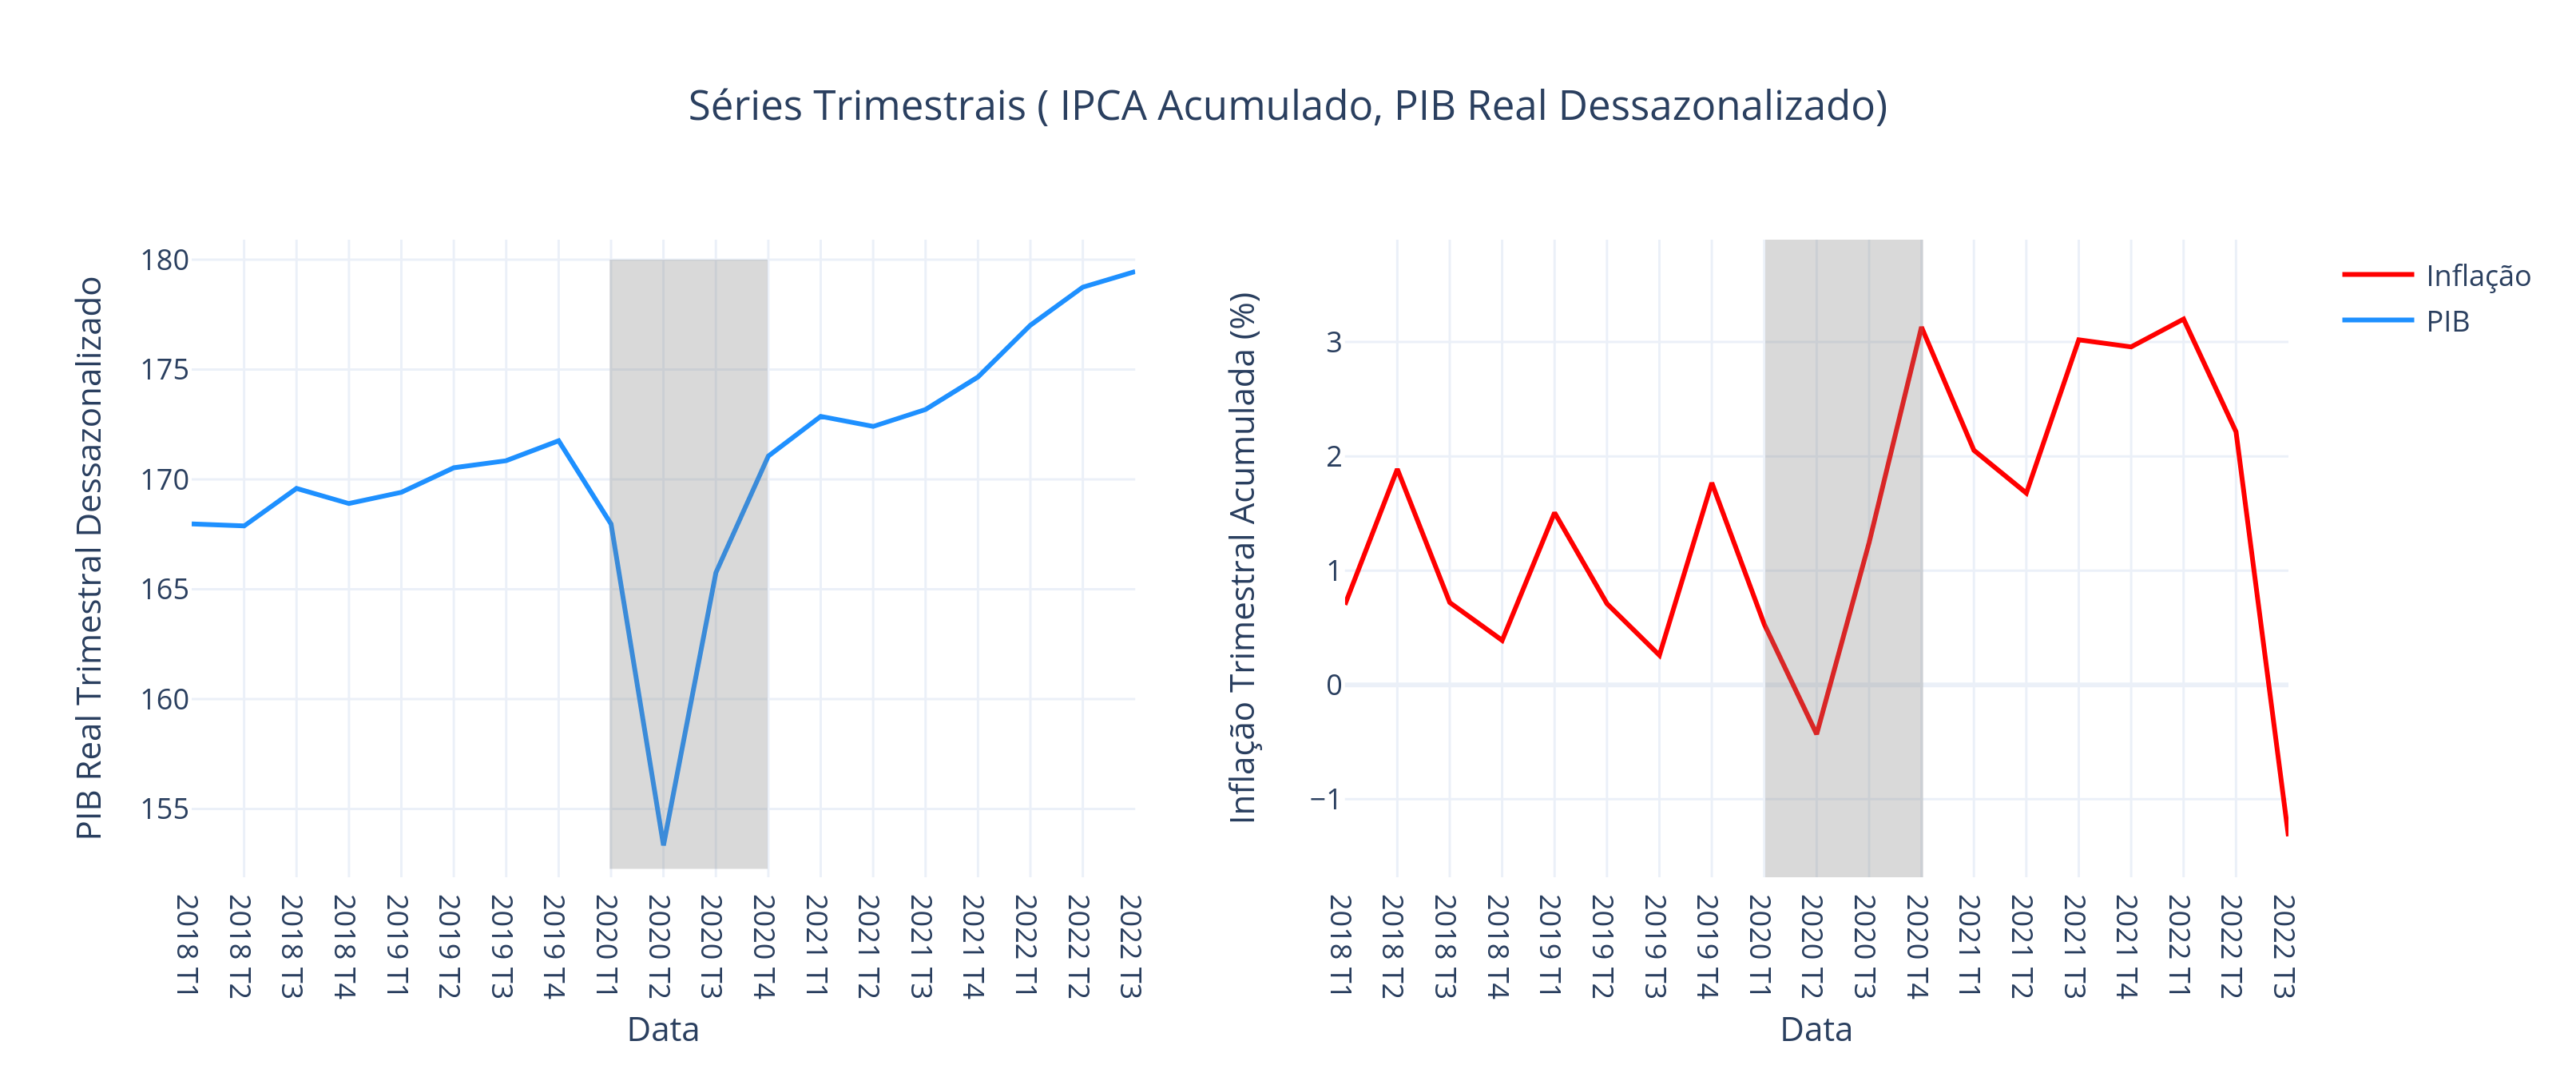
\includegraphics[width=1\columnwidth]{gráfico.png}
        % note that in above figure file name, "sr_setup",
        % the file extension is missing. LaTeX is smart enough to find
        % appropriate one (i.e. pdf, png, etc.)
        % You can add this extention yourself as it seen below
        % both notations are correct but above has more flexibility
        %\includegraphics[width=1.0\columnwidth]{sr_setup.pdf}
                \label{fig: Figura 6}
\end{figure}


De acordo com a figura 1, podemos notar que a partir do primeiro trimestre de 2020, com a chegada da pandemia, houve uma grande desaceleração econômica que ocasionou queda no PIB e inflação. Nesse mesmo período, a taxa Selic atingiu sua mínima histórica visando mitigar os efeitos do choque causado pela pandemia. Com isso, o PIB voltou a subir a partir do segundo trimestre de 2020. No entanto, a inflação subiu para além da meta naquele ano, o que fez com que o banco central posteriormente adotasse uma política monetária contracionista, visando convergir à meta. 



\closing{Presidente do Conselho Monetário Nacional}

%----------------------------------------------------------------------------------------

\end{letter}

\begin{letter}
{Tréplica em resposta do grupo composto por Emiliano Eustáquio, Felipe Cabral, Gabriel Pitta, João Oscar e Matheus Cavalcanti}

%----------------------------------------------------------------------------------------
%	LETTER CONTENT
%----------------------------------------------------------------------------------------
\opening{\textbf{Carta (problema) 2:}\\\\
Senhor Presidente,}

A adoção de uma política monetária mais restritiva a partir do ano de 2021 se fez necessária devido a uma pressão inflacionária que nos atingiu a partir do segundo semestre de 2020. Nesse sentido, é positivo perceber que o restante do Conselho Monetário Nacional compreende, em certa medida, que tal arrocho monetário é necessário em um momento de dificuldades.

Vale citar que também compreendemos a grande preocupação existente com o
elevado patamar em que a Selic se encontra, mas é importante ressaltar que isso se faz necessário em um momento em que ainda existem pressões inflacionárias que impedem, por momento, uma redução significativa na taxa de juros básica. Isso se torna ainda mais evidente quando percebemos que, mesmo com o patamar elevado da Selic, a inflação se encontra em um patamar acima da meta estabelecida pela CMN.

Assim como o restante do conselho, o Banco Central tem uma grande preocupação
com o crescimento econômico do país, e entendemos que a elevada taxa de juros pode ser um entrave para isso, mas salientamos que isso se faz necessário para que possamos ter um crescimento econômico sustentável e efetivo, já que uma redução na Selic por agora poderia elevar a inflação a um patamar muito acima do limite da meta, o que seria algo extremamente prejudicial, em especial para os mais pobres que são os mais afetados pela perda do poder de compra gerado pelo aumento nos preços.

Em síntese, cabe afirmar que o elevado patamar em que os juros se encontram,
apesar de ser um entrave para o desenvolvimento de curto prazo, se faz necessário para que o Brasil possa mantar a inflação sob controle e assim apresentar um desenvolvimento econômico de longo prazo sustentável.

\closing{Presidente do Banco Central do Brasil}

%----------------------------------------------------------------------------------------

\end{letter}
\end{document}